
\documentclass[12pt,a4paper]{article}
\usepackage[T2A]{fontenc}
\usepackage[utf8]{inputenc}
\usepackage[russian]{babel}
\usepackage{amsmath,amssymb}
\usepackage{geometry}
\usepackage{graphicx}
\usepackage{float}
\usepackage{booktabs}
\geometry{margin=2.2cm}

\title{Метод роя частиц для поиска минимума}
\author{}
\date{июнь 2026}

\begin{document}
\maketitle

\section*{Постановка}
Реализован алгоритм Particle Swarm Optimization для задачи
\[
J(x)\to\min,\qquad g_i(x)\le 0.
\]
В качестве демонстрационного примера использована двумерная задача
\[
J(x,y)=(x-1.2)^2+(y+1.4)^2+0.35\sin(2x)\cos(3y),
\]
\[
g_1=x^2+y^2-9\le 0,\qquad
 g_2=-x-y-2\le 0,\qquad
 g_3=x-2.5\le 0.
\]

\section*{Алгоритм}
На каждой итерации скорость частицы обновлялась по формуле
\[
v_k^{l+1}=\alpha_1v_k^l+\alpha_2r_2(x_k^{best}-x_k^l)+\alpha_3r_3(x^{best}-x_k^l),
\]
где $r_2,r_3\sim U[0,1]$. Затем вычислялось новое положение $x_k^{l+1}=x_k^l+v_k^{l+1}$.
Если новое положение нарушало ограничения, сначала выполнялось отражение скорости. Если отражённая точка также была недопустимой, частица оставалась в предыдущей допустимой позиции.

\section*{Параметры}
\begin{center}
\begin{tabular}{lr}
\toprule
Параметр & Значение \\
\midrule
Число частиц & 36 \\
Максимум итераций & 130 \\
$\alpha_1$ & 0.55 \\
$\alpha_2$ & 0.25 \\
$\alpha_3$ & 0.2 \\
Коэффициент отражения & 0.65 \\
\bottomrule
\end{tabular}
\end{center}

\section*{Результат}
\begin{center}
\begin{tabular}{lrrrl}
\toprule
Метод & $x$ & $y$ & $J(x,y)$ & останов \\
\midrule
PSO & 1.044388 & -1.199166 & -0.208479 & particle\_positions \\
Сеточная проверка & 1.042004 & -1.202312 & -0.208445 & reference \\
\bottomrule
\end{tabular}
\end{center}
Алгоритм выполнил 35 итераций. Сеточная проверка приведена только как ориентир для двумерного примера.

\section*{Графики}
\begin{figure}[H]
\centering
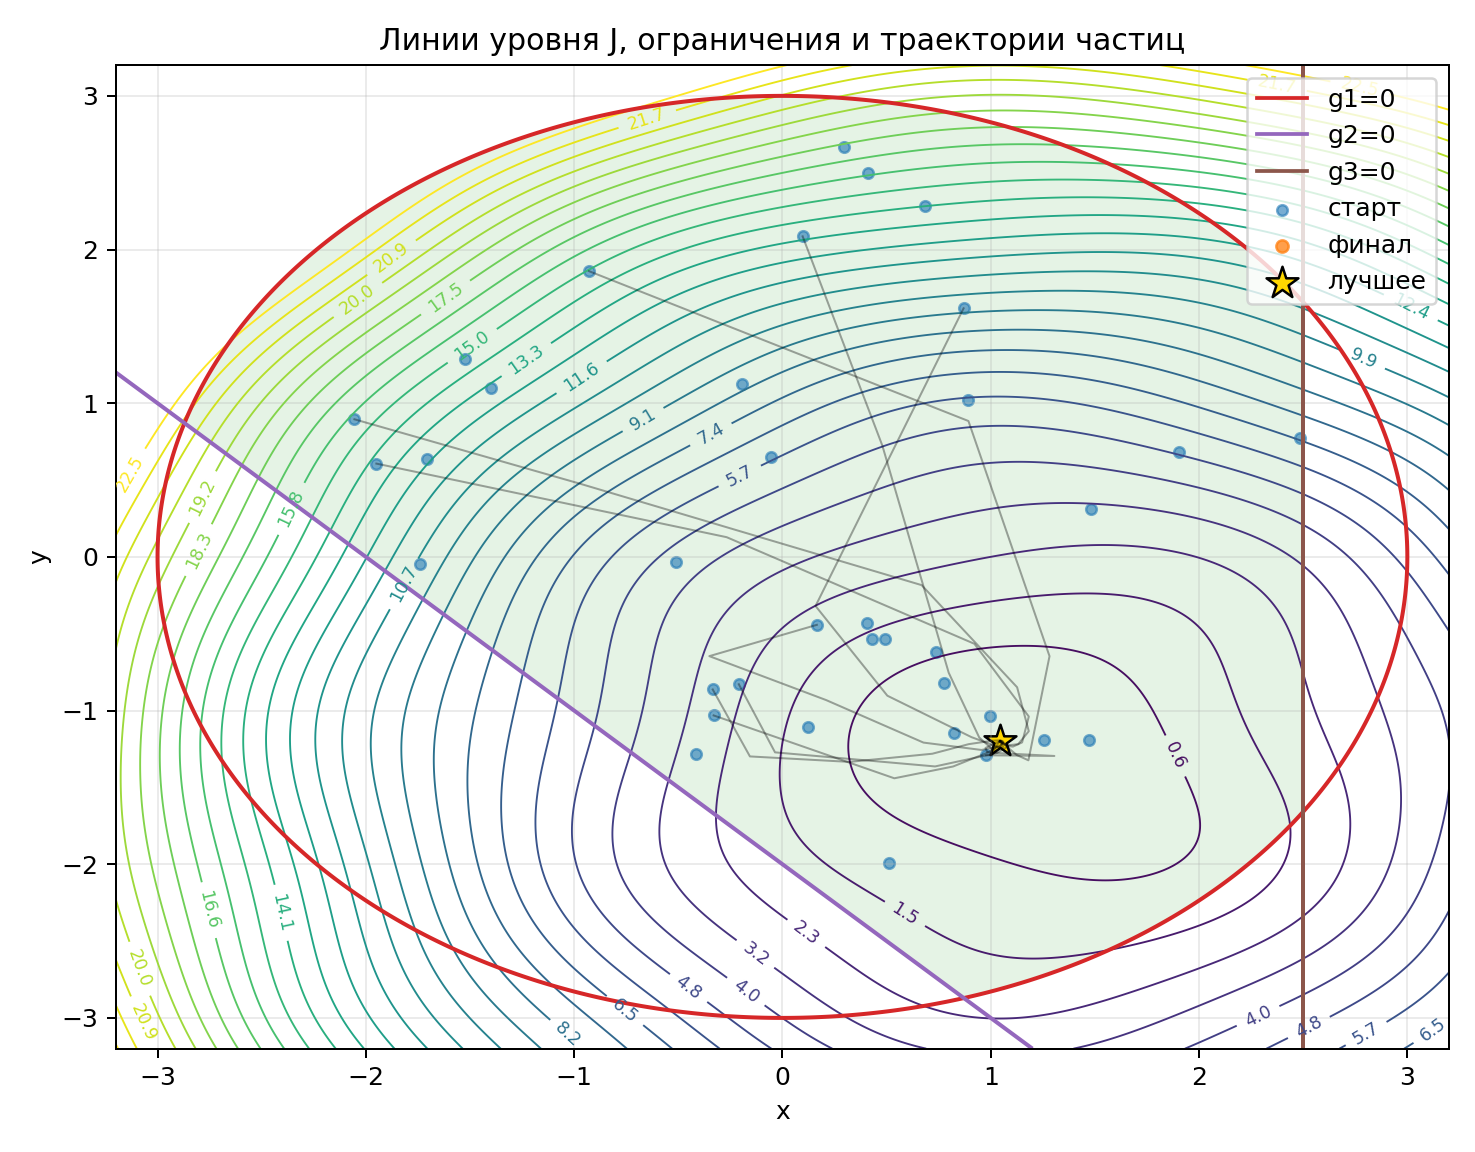
\includegraphics[width=0.9\textwidth]{graphs/pso_contours_trajectories.png}
\caption{Линии уровня функционала, границы ограничений и траектории частиц.}
\end{figure}

\begin{figure}[H]
\centering
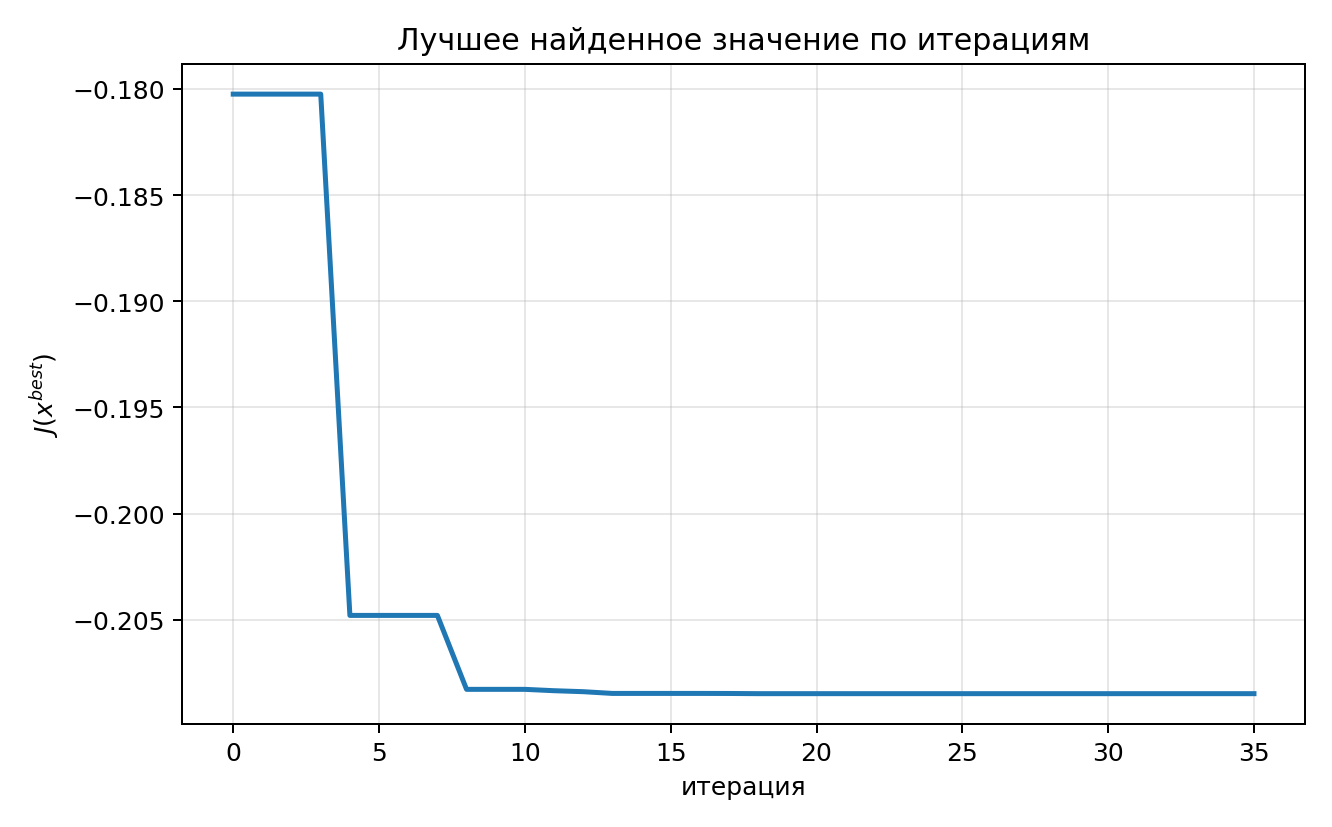
\includegraphics[width=0.82\textwidth]{graphs/pso_best_history.png}
\caption{Изменение лучшего найденного значения $J(x^{best})$ по итерациям.}
\end{figure}

\begin{figure}[H]
\centering
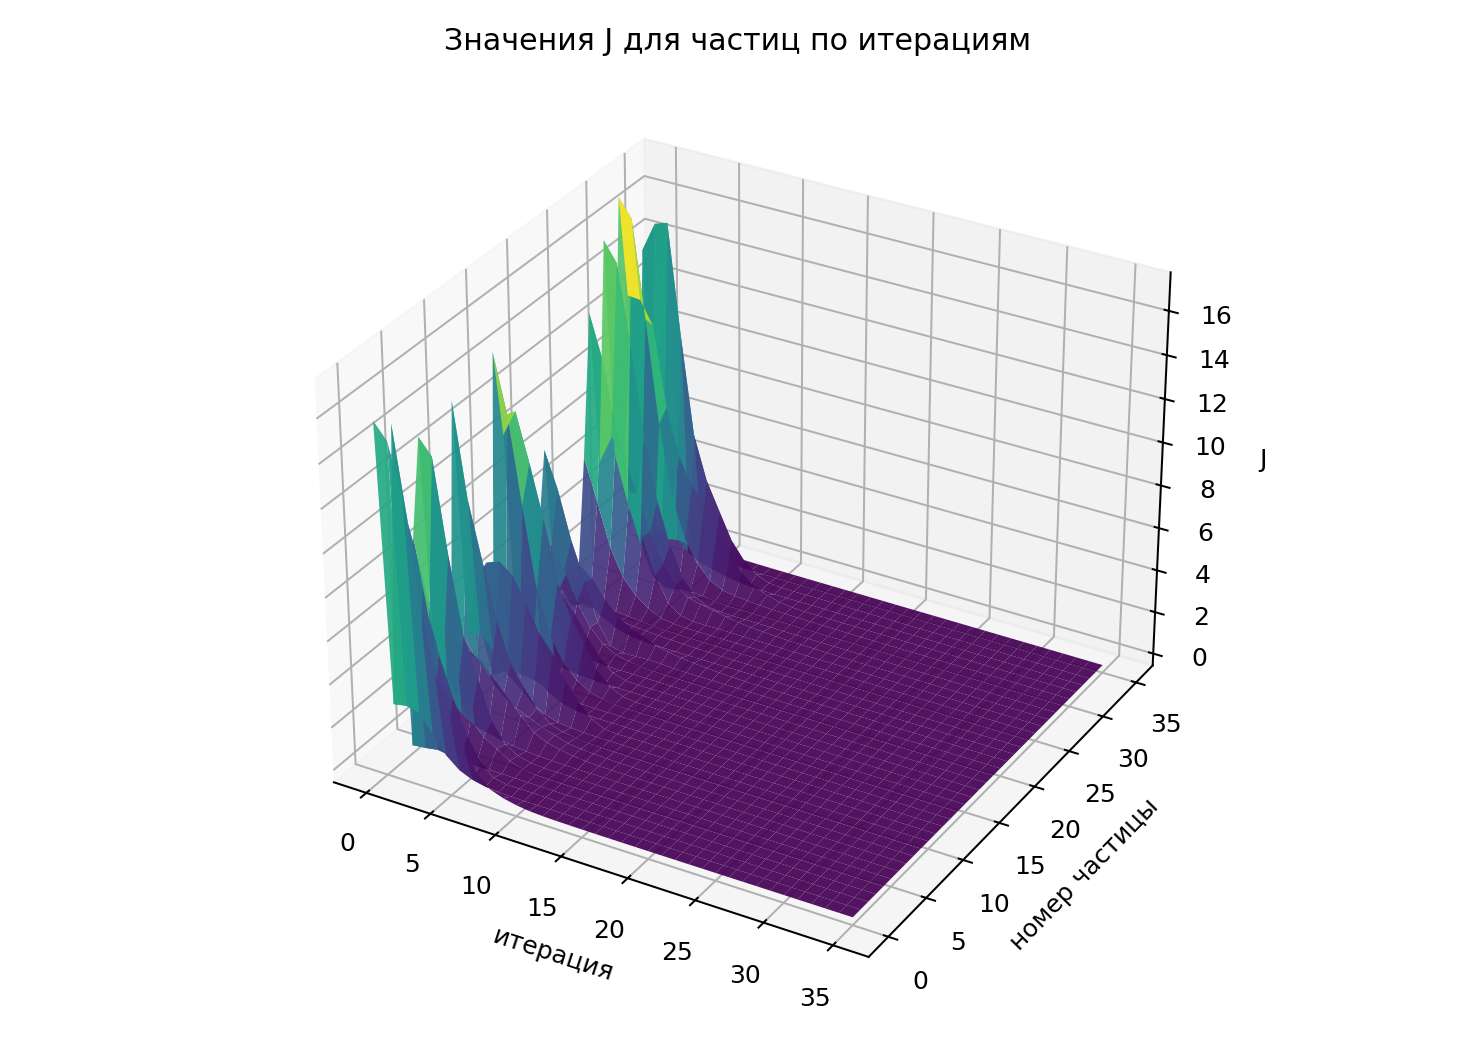
\includegraphics[width=0.9\textwidth]{graphs/pso_particle_value_surface.png}
\caption{Поверхность значений $J(x_k^l)$ по номеру итерации и номеру частицы.}
\end{figure}

\begin{figure}[H]
\centering
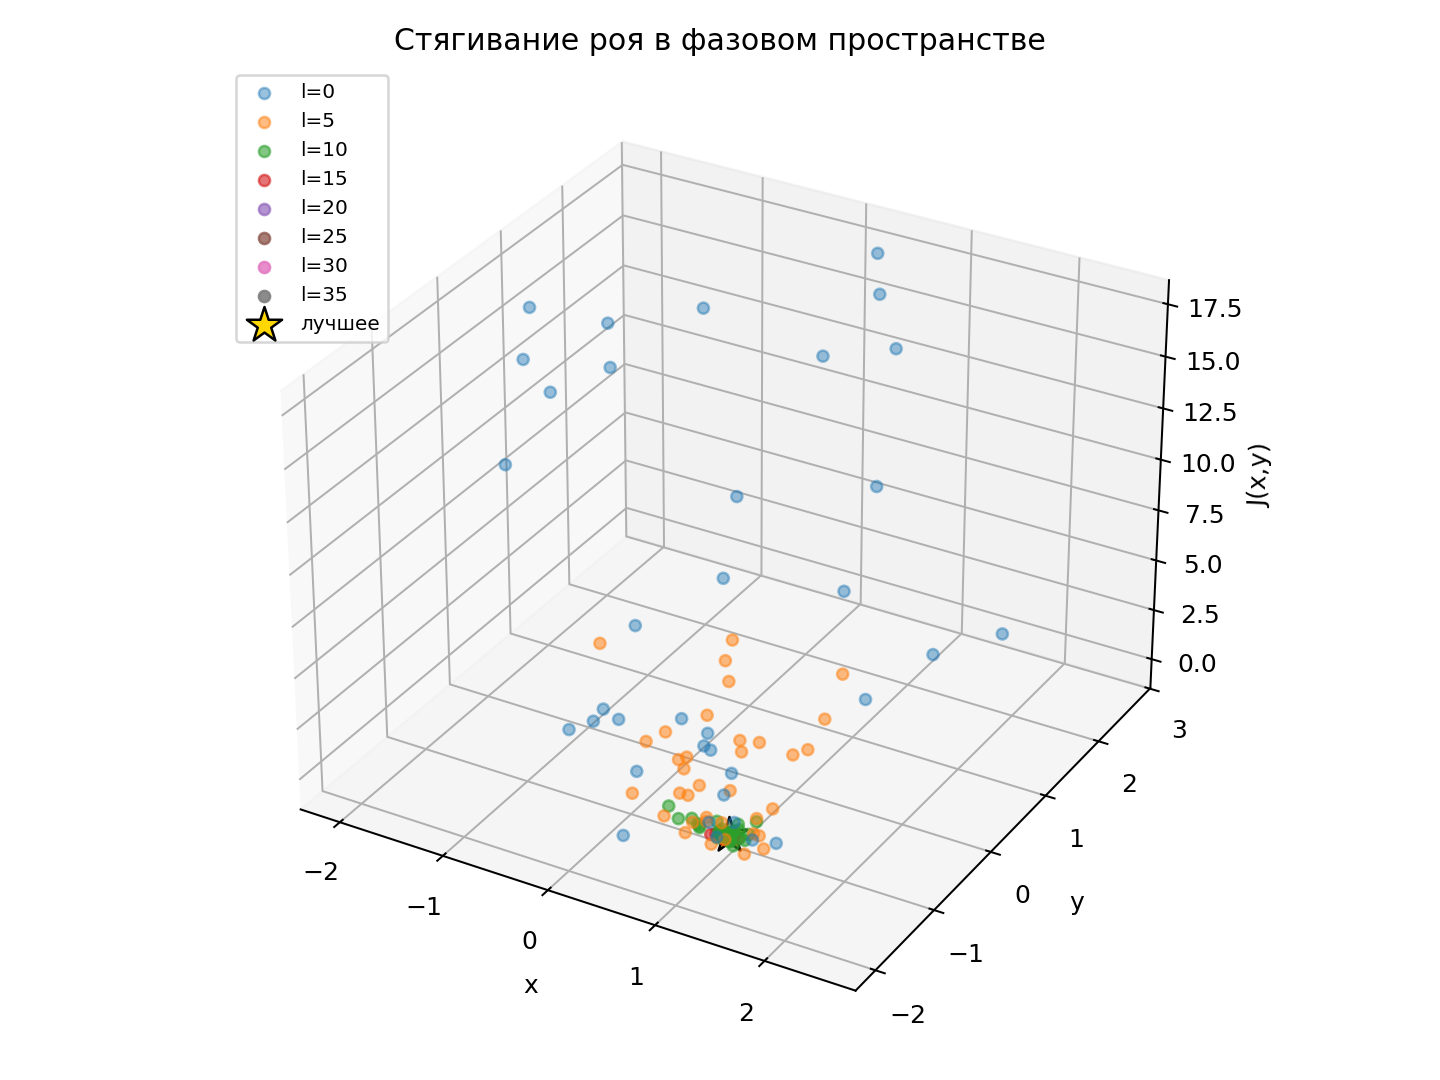
\includegraphics[width=0.9\textwidth]{graphs/pso_swarm_3d.png}
\caption{Стягивание частиц в фазовом пространстве $(x,y,J)$.}
\end{figure}

\section*{Вывод}
Метод роя частиц устойчиво нашёл допустимую точку минимума. Механизм отражения не допускает ухода частиц за границы области, а графики показывают сходимость лучшего значения и концентрацию роя около найденного экстремума.

\end{document}
